\documentclass[10pt]{article}
\usepackage{tikz}
\usepackage[margin=0cm]{geometry}
\pagestyle{empty}

\begin{document}

\vspace*{\fill}
\begin{center}
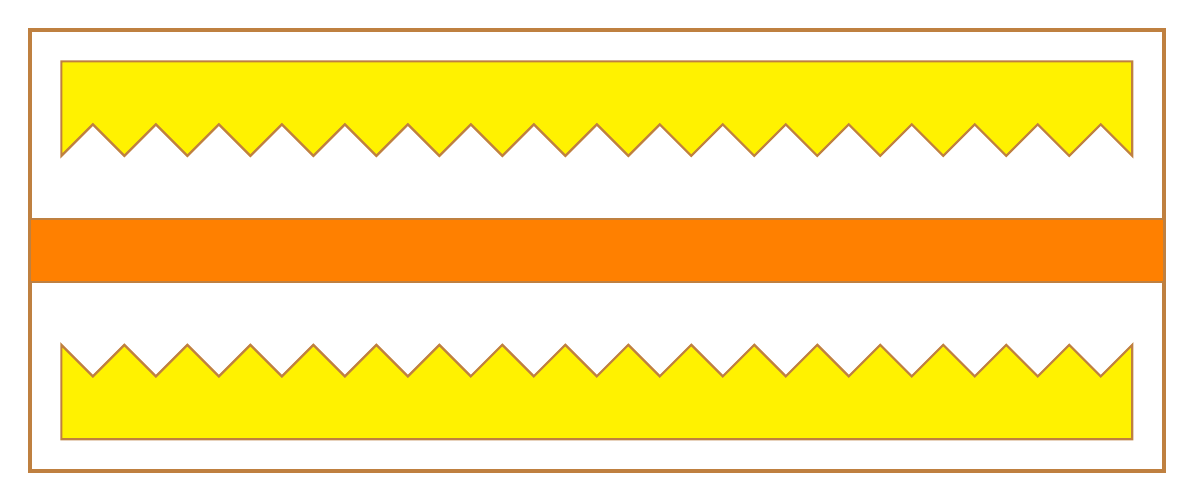
\begin{tikzpicture}[x=0.4cm, y=-0.4cm, thick, brown]
\draw[ultra thick] (0, 0) -- (36, 0) -- (36, 14) -- (0, 14) -- cycle;
%Depth 0
\filldraw[fill=orange!0!yellow] (1, 1) -- (35, 1) -- (35, 4) -- (34, 3) -- (33, 4) -- (32, 3) -- (31, 4) -- (30, 3) -- (29, 4) -- (28, 3) -- (27, 4) -- (26, 3) -- (25, 4) -- (24, 3) -- (23, 4) -- (22, 3) -- (21, 4) -- (20, 3) -- (19, 4) -- (18, 3) -- (17, 4) -- (16, 3) -- (15, 4) -- (14, 3) -- (13, 4) -- (12, 3) -- (11, 4) -- (10, 3) -- (9, 4) -- (8, 3) -- (7, 4) -- (6, 3) -- (5, 4) -- (4, 3) -- (3, 4) -- (2, 3) -- (1, 4) -- cycle;
\filldraw[fill=orange!100!yellow] (0, 6) -- (36, 6) -- (36, 8) -- (0, 8) -- cycle;
\filldraw[fill=orange!0!yellow] (1, 10) -- (2, 11) -- (3, 10) -- (4, 11) -- (5, 10) -- (6, 11) -- (7, 10) -- (8, 11) -- (9, 10) -- (10, 11) -- (11, 10) -- (12, 11) -- (13, 10) -- (14, 11) -- (15, 10) -- (16, 11) -- (17, 10) -- (18, 11) -- (19, 10) -- (20, 11) -- (21, 10) -- (22, 11) -- (23, 10) -- (24, 11) -- (25, 10) -- (26, 11) -- (27, 10) -- (28, 11) -- (29, 10) -- (30, 11) -- (31, 10) -- (32, 11) -- (33, 10) -- (34, 11) -- (35, 10) -- (35, 13) -- (1, 13) -- cycle;
\end{tikzpicture}
\end{center}
\vspace*{\fill}

\end{document}
